\huaxing{夯基达标}{基础巩固\quad 稳拿保分}

\jx{1}{源 1.1.1.5-4·简单}{有下列说法:\hfill\kylabel{（知识点3）}}

\bindopt ①若\(\overrightarrow{p} = x\overrightarrow{a} + y\overrightarrow{b}\)，则\(\overrightarrow{p}\)与\(\overrightarrow{a}\)，\(\overrightarrow{b}\)共面；②若\(\overrightarrow{p}\)与\(\overrightarrow{a}\)，\(\overrightarrow{b}\)共面，则\(\overrightarrow{p}\)=\emph{x}\(\overrightarrow{a}\)+\emph{y}\(\overrightarrow{b}\)；③若\(\overrightarrow{MP}\)=\emph{x}\(\overrightarrow{MA}\)+\emph{y}\(\overrightarrow{MB}\)，则\emph{P}，\emph{M}，\emph{A}，\emph{B}共面；④若\emph{P}，\emph{M}，\emph{A}，\emph{B}共面，则\(\overrightarrow{MP}\)=\emph{x}\(\overrightarrow{MA}\)+\emph{y}\(\overrightarrow{MB}\).其中正确的是（~~~~）

\bindopt A．①②③④；B．①③④；C．①③；D．②④

\huaxing{提能进阶}{综合应用\quad 进阶提分}

\jx{2}{源 1.1.1.7-6·中档}{如图，在正方体\hfill\kylabel{（知识点3）}\\\(ABCD - A_{1}B_{1}C_{1}D_{1}\)中，求向量\(\overrightarrow{BC_{1}}\)与\(\overrightarrow{AC}\)的夹角的大小．}

\bindp \penalty10000\hangindent=0pt\hangafter=1\noindent\hspace*{7mm}\makebox[\dimexpr\linewidth-7mm\relax][c]{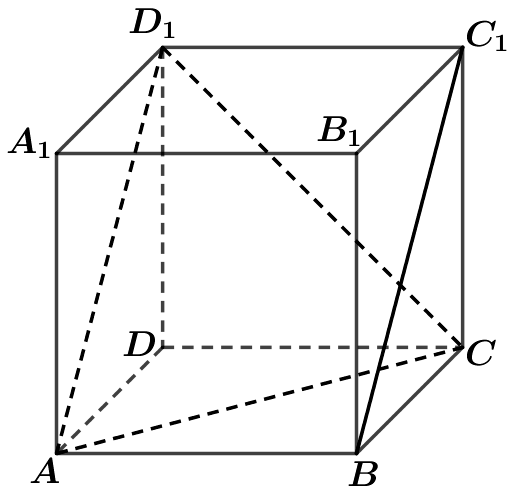
\includegraphics[width=30mm,alt={@@@d8ffc038-cfd6-4d16-b846-f3d81f29b325}]{media/media/image3.png}}\par\penalty10000

\jx{3}{源 1.1.1.9-9·中档}{如图，在大小为45°\hfill\kylabel{（知识点3）}\\的二面角A\-EF\-D中，四边形ABFE，CDEF都是边长为1的正方形，则B，D两点间的距离是()}

\bindp \penalty10000\hangindent=0pt\hangafter=1\noindent\hspace*{7mm}\makebox[\dimexpr\linewidth-7mm\relax][c]{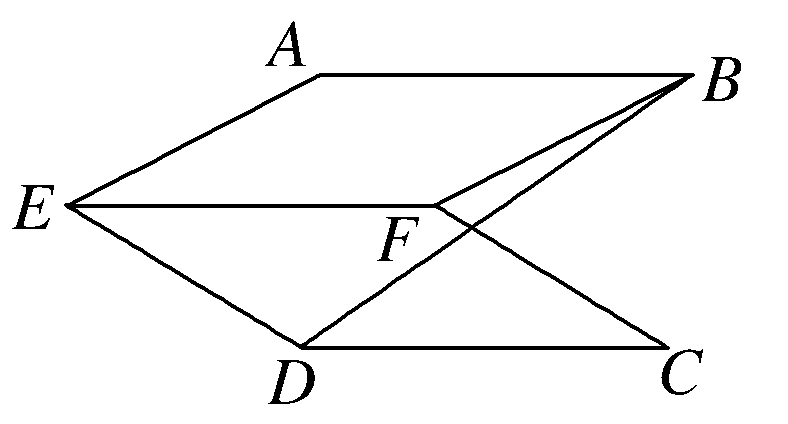
\includegraphics[width=30mm,alt={@@@494a628b97d74c2894c135f69e8f1eb7}]{media/media/image4.png}}\par\penalty10000

\bindopt A．\(\sqrt{3}\)；B．\(\sqrt{2}\)；C．1；D．\(\sqrt{3 - \sqrt{2}}\)

\jx{4}{源 1.1.1.10-10·中档}{已知矩形\(ABCD\)中，\hfill\kylabel{（知识点3）}\\\(AB = 1\)，\(BC = \sqrt{3}\)，将矩形\(ABCD\)沿对角线\(AC\)折起，使平面\(ABC\)与平面\(ACD\)垂直，则\(|\overrightarrow{BD}| =\)（~~~~）．}

\bindopt A．\(\frac{\sqrt{10}}{2}\)；B．\(\frac{\sqrt{6}}{2}\)；C．\(\frac{\sqrt{5}}{2}\)；D．2
